\documentclass{beamer}
\mode<presentation>
\usetheme{CambridgeUS}
\usepackage[russian]{babel}
\usepackage[utf8]{inputenc}
\usepackage[T2A]{fontenc}
\usepackage{sansmathaccent}

\usepackage{verbatim}
\usepackage{alltt}

\pdfmapfile{+sansmathaccent.map}
\title[Шаблоны]{Шаблоны информационной архитектуры}
\author{Наумов Д.А., доц. каф. КТ}
\date[18.11.2020] {Компьютерная графика и проектирование графических интерфейсов, 2020}

\begin{document}

%ТИТУЛЬНЫЙ СЛАЙД
\begin{frame}
  \titlepage
\end{frame}
  
%СОДЕРЖАНИЕ ЛЕКЦИИ
\begin{frame}
  \frametitle{Содержание лекции}
  \tableofcontents  
\end{frame}

\section{Информационная архитектура, организация контента}

\begin{frame}[t]
	\textit{Высокоуровневая оганизация информации:}
	\begin{itemize}
		\item разделение сущностей -- отделение содержимого от физического представления;
		\item физическая структура -- представление материала на страницах.
	\end{itemize}
	
	Большинство приложений и многие веб-сайты организуются соглласно одному из нескольких следующих принципов:
	\begin{itemize}
		\item \textit{списки объектов} -- папка входящих сообщений;
		\item \textbf{списки действий или задач} -- посмотреть, приобрести, продать, зарегистрироваться; 		
		\item \textit{списки тематических категорий} -- здоровье, наука, технология;		
		\item \textit{списки инструментов} -- календарь, адресная книга, блокнот.		
	\end{itemize}
	
	Любую страницу можно рассматривать с точки зрения того, что оно долнжа делать:
	\begin{itemize}
		\item отобразить едиственный объект (карта, книга, видео, игра);
		\item отобразить список объектов;
		\item \textbf{предоставить возможность что-то сделать};
		\item \textbf{выполнить определенную задачу}.				
	\end{itemize}
\end{frame} 

\section{Действия и команды}

\begin{frame}[t]{Direct object manipulation}
	\begin{figure}[h]
		\centering
		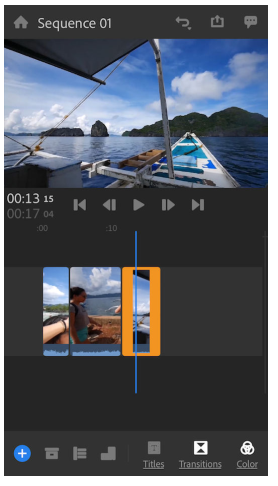
\includegraphics[scale=0.5]{images/lec08-pic01.png}
	\end{figure}
\end{frame}	

\begin{frame}[t]{Button Groups}
	\begin{figure}[h]
		\centering
		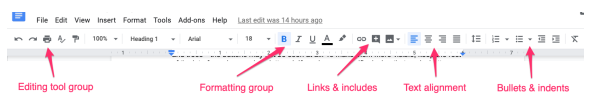
\includegraphics[scale=0.6]{images/lec08-pic02.png}
		\caption{Button Groups in Google Docs}
	\end{figure}
	\begin{figure}[h]
		\centering
		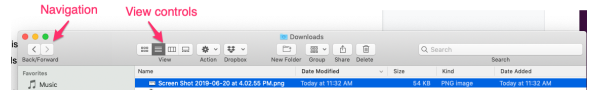
\includegraphics[scale=0.6]{images/lec08-pic03.png}
		\caption{Apple macOS Finder}
	\end{figure}	
\end{frame}	

\begin{frame}[t]{Hover or Pop-Up Tools}
	\begin{figure}[h]
		\centering
		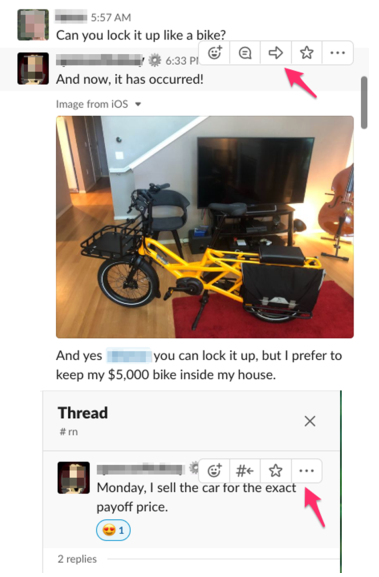
\includegraphics[scale=0.6]{images/lec08-pic04.png}
		\caption{Slack; examples of hover tools for posts and threads}
	\end{figure}
\end{frame}	

\begin{frame}[t]{Hover or Pop-Up Tools}
	\begin{figure}[h]
		\centering
		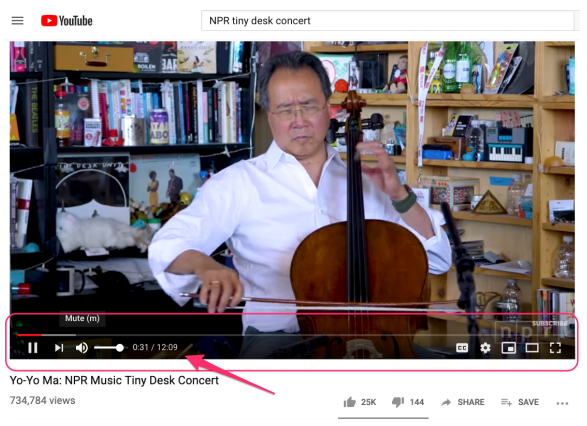
\includegraphics[scale=0.6]{images/lec08-pic05.png}
		\caption{YouTube web player}
	\end{figure}
\end{frame}

\begin{frame}[t]{Action Panel}
	\begin{figure}[h]
		\centering
		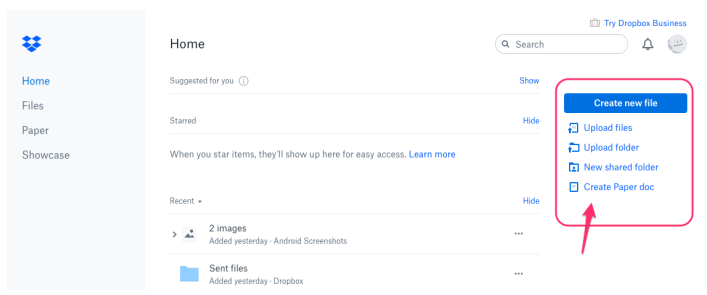
\includegraphics[scale=0.6]{images/lec08-pic06.png}
		\caption{An Action Panel in Dropbox}
	\end{figure}
\end{frame}

\begin{frame}[t]{Action Panel}
	\begin{figure}[h]
		\centering
		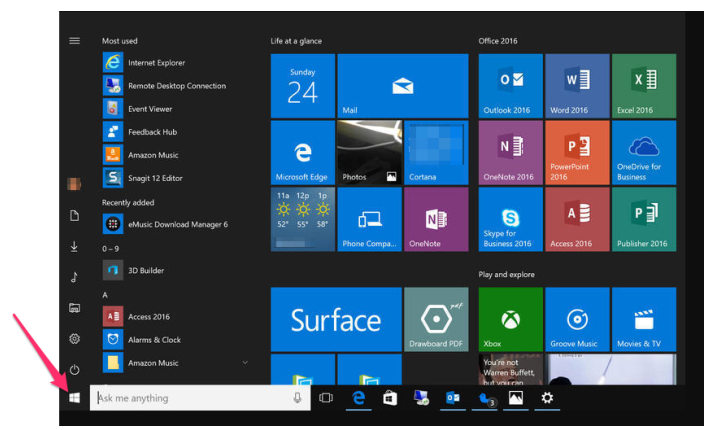
\includegraphics[scale=0.6]{images/lec08-pic07.png}
		\caption{Microsof Windows 10 Start Menu}
	\end{figure}
\end{frame}

\begin{frame}[t]{Action Panel}
	\begin{figure}[h]
		\centering
		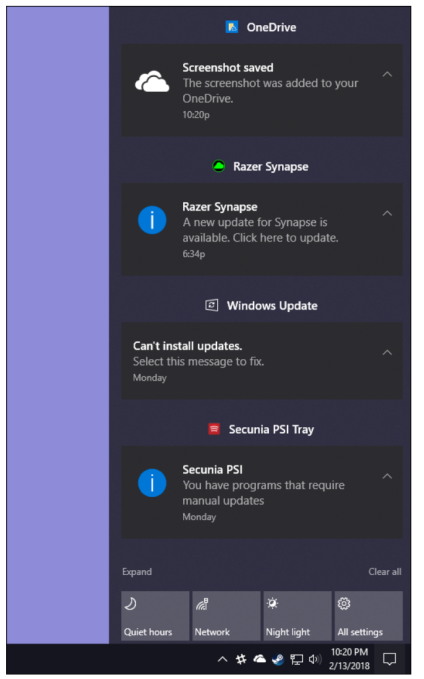
\includegraphics[scale=0.6]{images/lec08-pic08.png}
		\caption{Microsof Windows 10 Action Panel}
	\end{figure}
\end{frame}

\begin{frame}[t]{Prominent <<Done>> Button or Assumed Next Step}
	\begin{figure}[h]
		\centering
		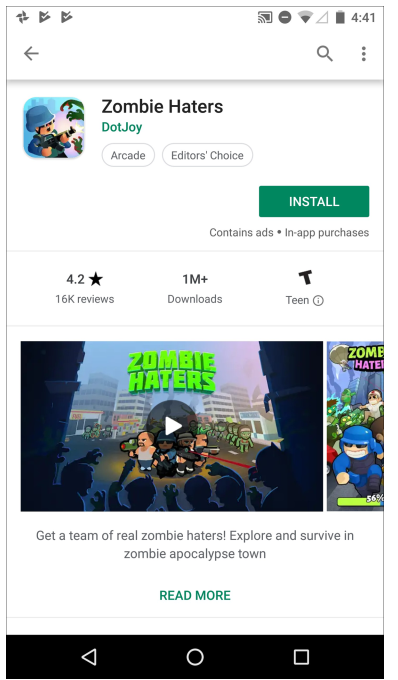
\includegraphics[scale=0.6]{images/lec08-pic09.png}
		\caption{Google Play store, Android OS mobile device}
	\end{figure}
\end{frame}

\begin{frame}[t]{Prominent <<Done>> Button or Assumed Next Step}
	\begin{figure}[h]
		\centering
		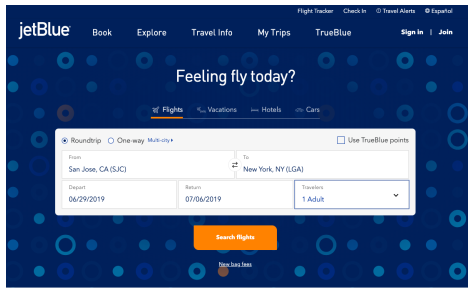
\includegraphics[scale=0.6]{images/lec08-pic10.png}
		\caption{JetBlue.com}
	\end{figure}
\end{frame}

\begin{frame}[t]{Prominent <<Done>> Button or Assumed Next Step}
	\begin{figure}[h]
		\centering
		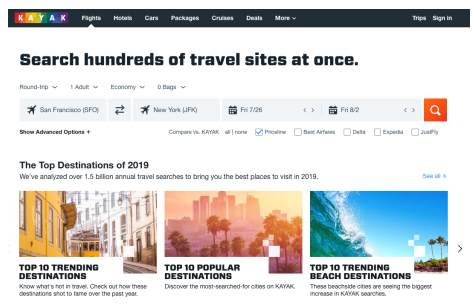
\includegraphics[scale=0.6]{images/lec08-pic11.png}
		\caption{Kayak.com}
	\end{figure}
\end{frame}

\begin{frame}[t]{Prominent <<Done>> Button or Assumed Next Step}
	\begin{figure}[h]
		\centering
		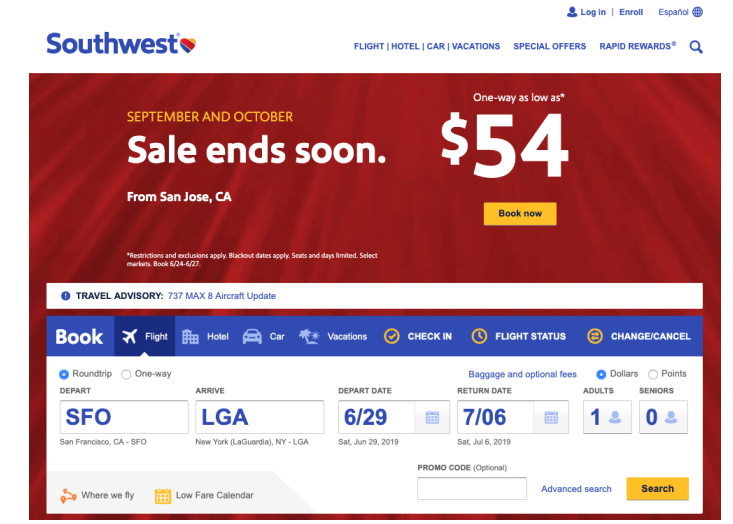
\includegraphics[scale=0.6]{images/lec08-pic12.png}
		\caption{Southwest.com}
	\end{figure}
\end{frame}

\begin{frame}[t]{Prominent <<Done>> Button or Assumed Next Step}
	\begin{figure}[h]
		\centering
		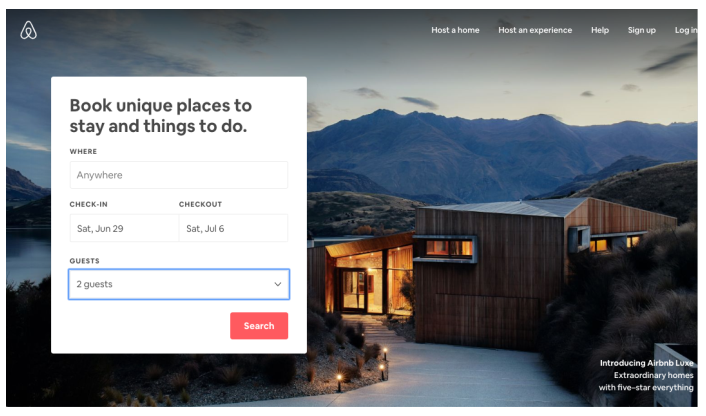
\includegraphics[scale=0.6]{images/lec08-pic13.png}
		\caption{Airbnb.com}
	\end{figure}
\end{frame}

\begin{frame}[t]{Smart Menu Items}
	\begin{figure}[h]
		\centering
		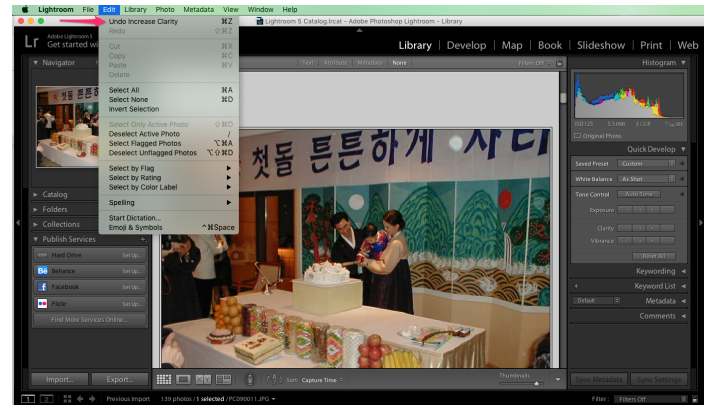
\includegraphics[scale=0.6]{images/lec08-pic14.png}
		\caption{Adobe Lightroom}
	\end{figure}
\end{frame}

\begin{frame}[t]{Smart Menu Items}
	\begin{figure}[h]
		\centering
		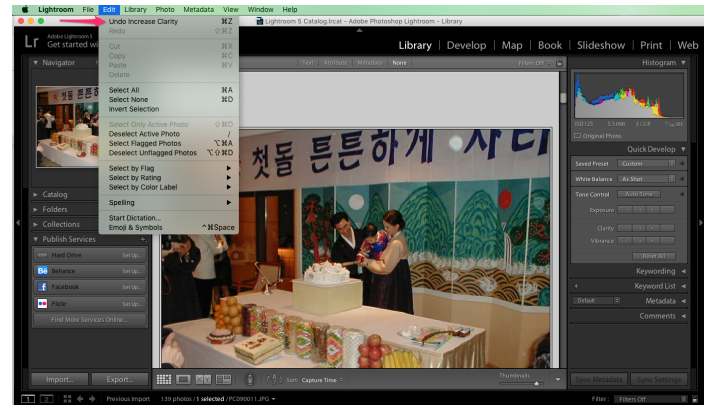
\includegraphics[scale=0.6]{images/lec08-pic14.png}
		\caption{Adobe Lightroom}
	\end{figure}
\end{frame}

\begin{frame}[t]{Smart Menu Items}
	\begin{figure}[h]
		\centering
		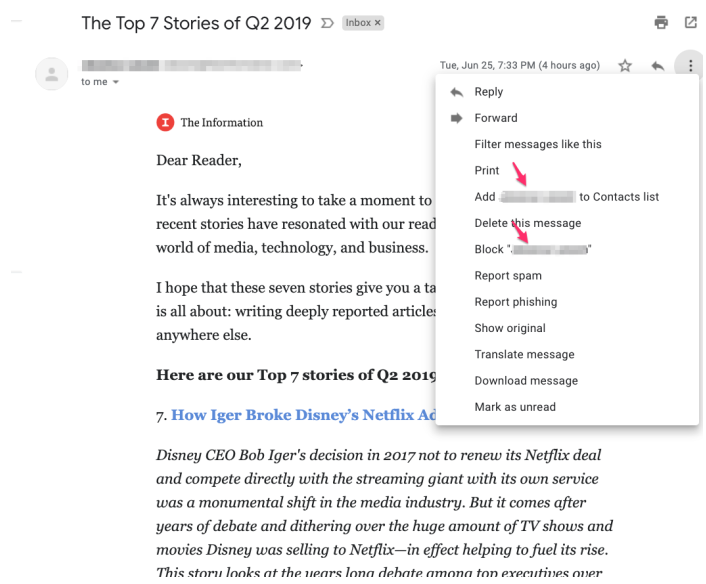
\includegraphics[scale=0.6]{images/lec08-pic15.png}
		\caption{GMail}
	\end{figure}
\end{frame}

\begin{frame}[t]{Preview}
	\begin{figure}[h]
		\centering
		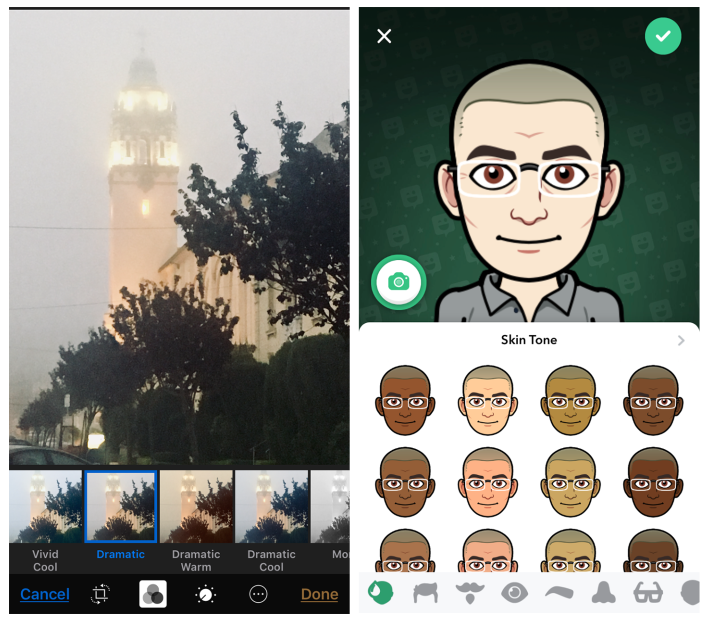
\includegraphics[scale=0.6]{images/lec08-pic16.png}
		\caption{Apple Photos app and Bitmoji app}
	\end{figure}
\end{frame}

\begin{frame}[t]{Preview}
	\begin{figure}[h]
		\centering
		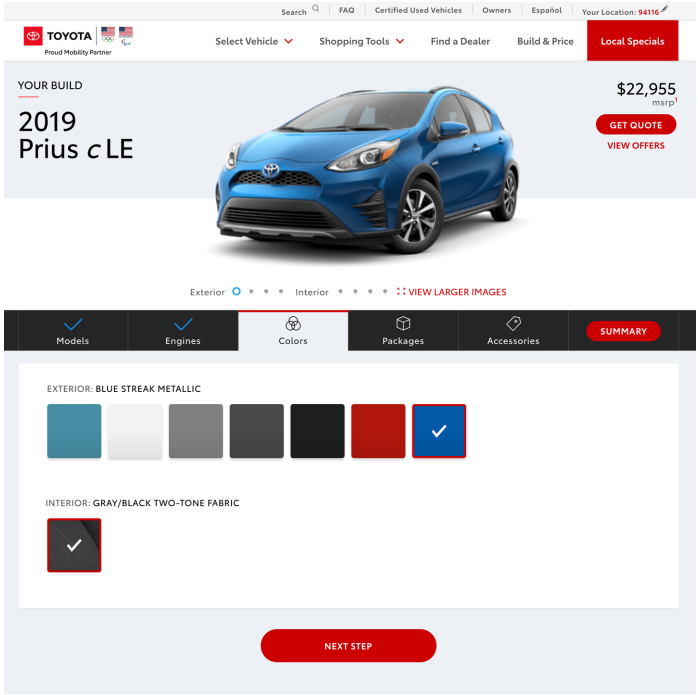
\includegraphics[scale=0.6]{images/lec08-pic17.png}
		\caption{Toyota.com}
	\end{figure}
\end{frame}

\begin{frame}[t]{Preview}
	\begin{figure}[h]
		\centering
		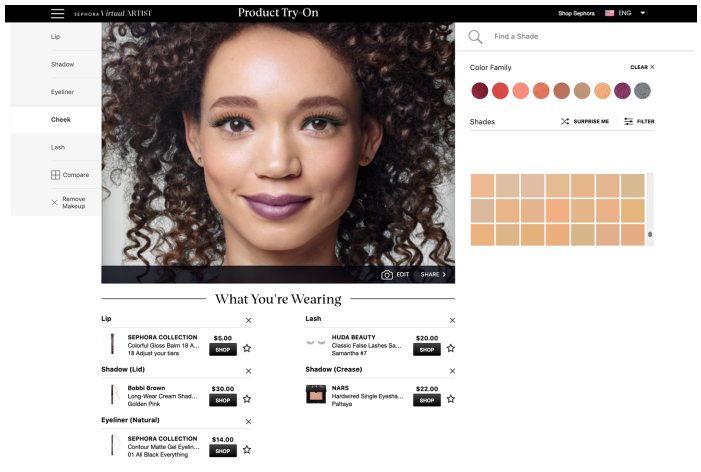
\includegraphics[scale=0.6]{images/lec08-pic18.png}
		\caption{Sephora.com}
	\end{figure}
\end{frame}

\begin{frame}[t]{Spinners and Loading Indicators}
	\begin{figure}[h]
		\centering
		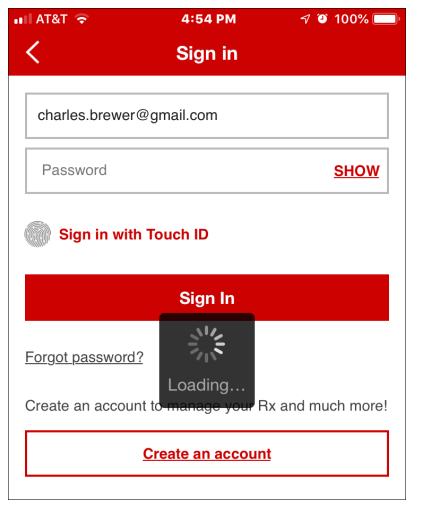
\includegraphics[scale=0.6]{images/lec08-pic19.png}
		\caption{Apple iOS, CVS mobile app; An iOS spinner example}
	\end{figure}
\end{frame}

\begin{frame}[t]{Spinners and Loading Indicators}
	\begin{figure}[h]
		\centering
		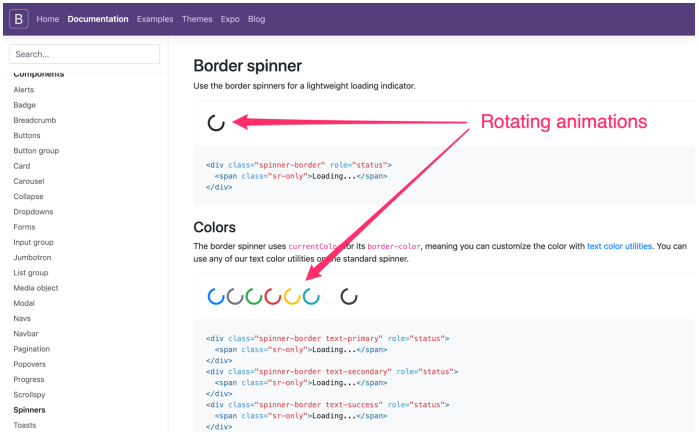
\includegraphics[scale=0.6]{images/lec08-pic20.png}
		\caption{Twitter Bootstrap component library (getbootstrap.com) border spinner}
	\end{figure}
\end{frame}

\begin{frame}[t]{Spinners and Loading Indicators}
	\begin{figure}[h]
		\centering
		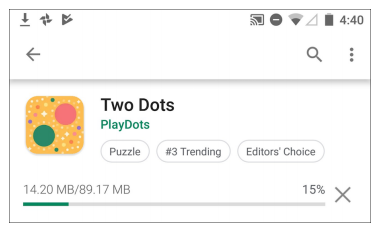
\includegraphics[scale=0.6]{images/lec08-pic21.png}
		\caption{Adobe Creative Cloud desktop manager, macOS}
	\end{figure}
\end{frame}

\begin{frame}[t]{Cancelability}
	\begin{figure}[h]
		\centering
		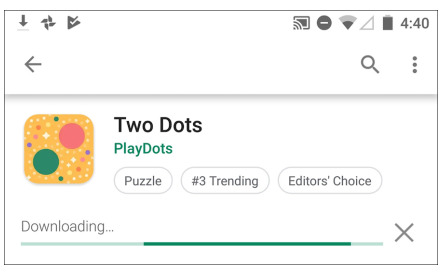
\includegraphics[scale=0.6]{images/lec08-pic22.png}
		\caption{Google Play store, Android OS}
	\end{figure}
\end{frame}

\begin{frame}[t]{Cancelability}
	\begin{figure}[h]
		\centering
		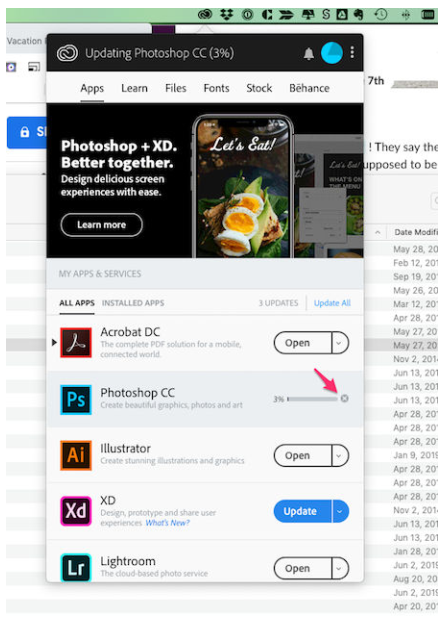
\includegraphics[scale=0.6]{images/lec08-pic23.png}
		\caption{Adobe Creative Cloud desktop manager, macOS}
	\end{figure}
\end{frame}

\begin{frame}[t]{Multilevel Undo}
	\begin{figure}[h]
		\centering
		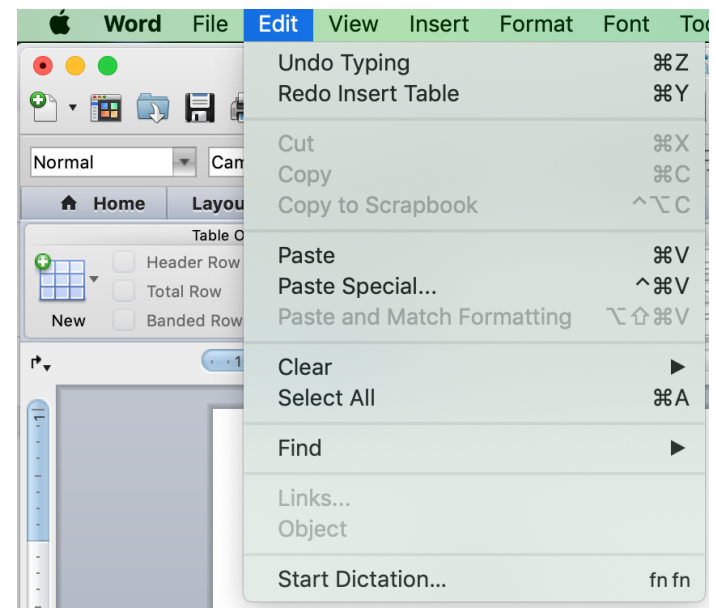
\includegraphics[scale=0.6]{images/lec08-pic24.png}
		\caption{Microsof Word History of Actions}
	\end{figure}
\end{frame}

\begin{frame}[t]{Command History}
	\begin{figure}[h]
		\centering
		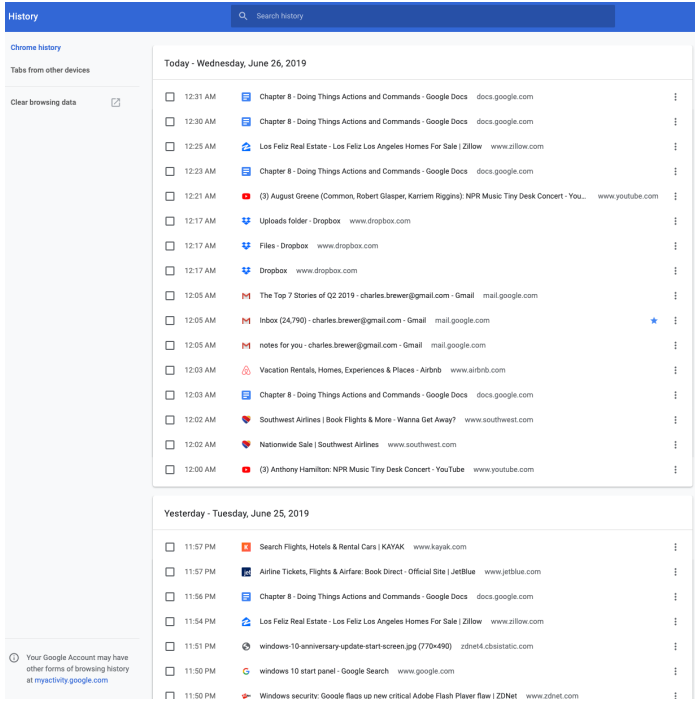
\includegraphics[scale=0.6]{images/lec08-pic25.png}
		\caption{Google Chrome History screen}
	\end{figure}
\end{frame}

\begin{frame}[t]{Command History}
	\begin{figure}[h]
		\centering
		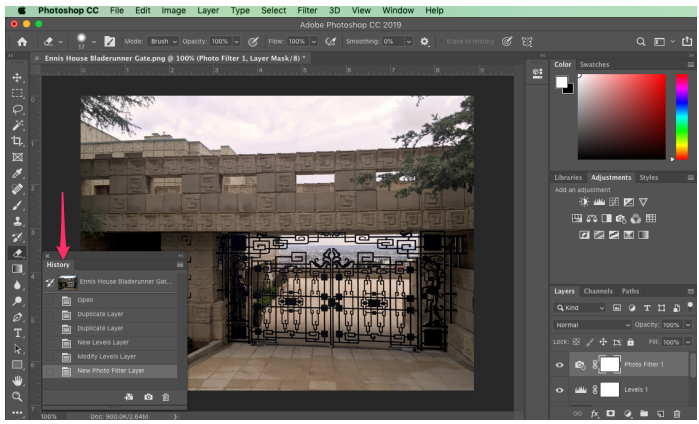
\includegraphics[scale=0.6]{images/lec08-pic26.png}
		\caption{Adobe Photoshop CC}
	\end{figure}
\end{frame}

\begin{frame}[t]{Macros}
	\begin{figure}[h]
		\centering
		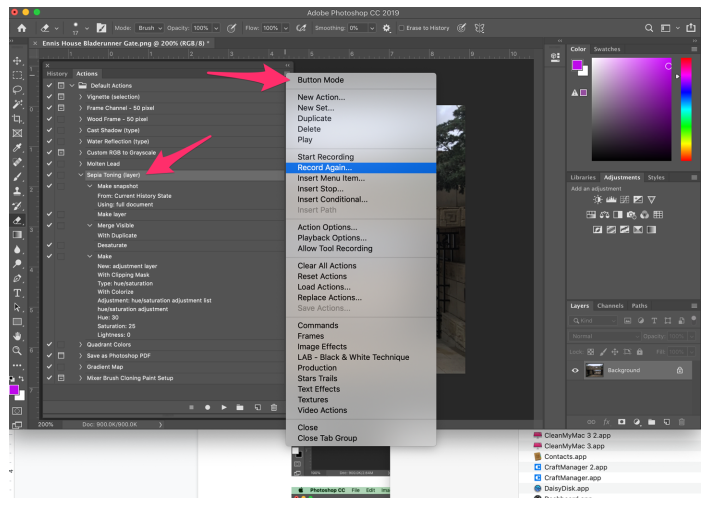
\includegraphics[scale=0.6]{images/lec08-pic27.png}
		\caption{Recording a macro in Adobe Photoshop CC}
	\end{figure}
\end{frame}

\begin{frame}[t]{Macros}
	\begin{figure}[h]
		\centering
		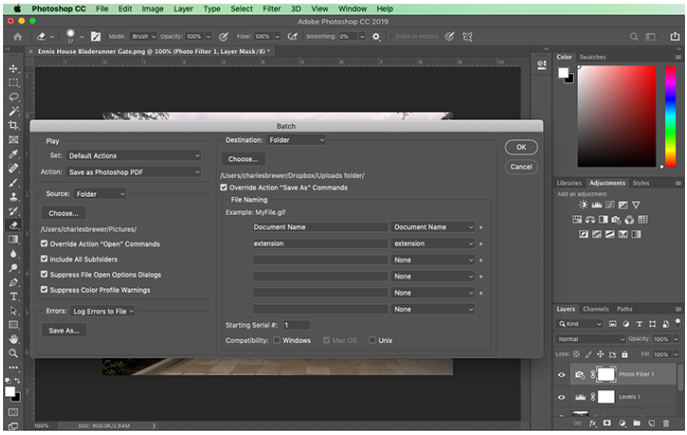
\includegraphics[scale=0.6]{images/lec08-pic28.png}
		\caption{Batch automation: confguring a series of actions to perform on multiple files automatically}
	\end{figure}
\end{frame}

\begin{frame}[t]{Macros}
	\begin{figure}[h]
		\centering
		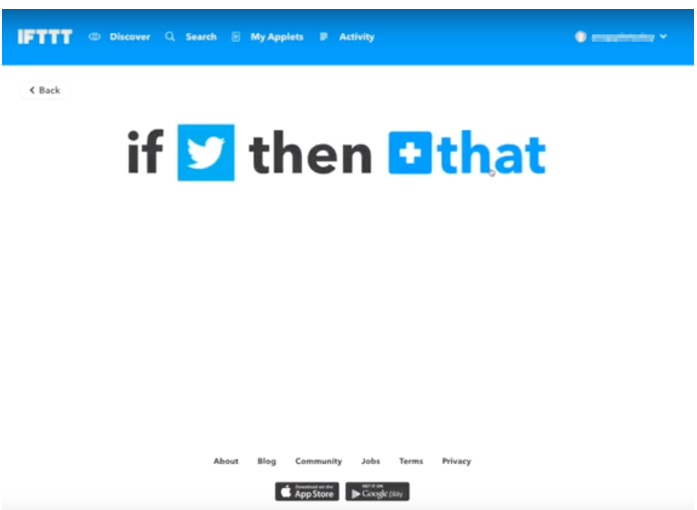
\includegraphics[scale=0.6]{images/lec08-pic29.png}
		\caption{IFTTT applet creator}
	\end{figure}
\end{frame}

\section{Формы и элементы управления}

%Respect the user’s time and attention
%Make sure the user understands the purpose of the form
%Minimize the number of form inputs
%Minimize visual clutter
%Group and title the form elements into sections where possible
%Consider dynamic, show/hide sections for long, complicated forms
%Use alignment for clear vertical flow
%Indicate what are required and what are optional felds
%Labels, instructions, examples, and help
%Use the width of the input felds to preview the length of the input
%Accept variations in input formatting
%Error prevention and validation as quickly as possible
%Consider top-aligned labels for mobile and web-responsive designs
%Consider internationalization
%Message success
%Usability test it

\begin{frame}[t]{Forgiving Format}
	\begin{figure}[h]
		\centering
		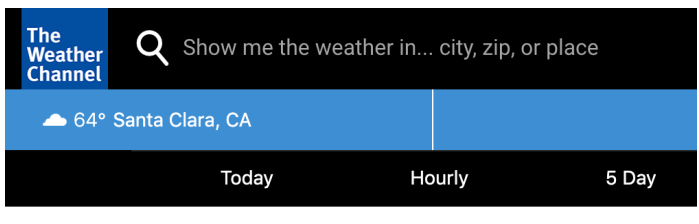
\includegraphics[scale=0.6]{images/lec08-pic30.png}
		\caption{Weather.com}
	\end{figure}
	
	\begin{figure}[h]
		\centering
		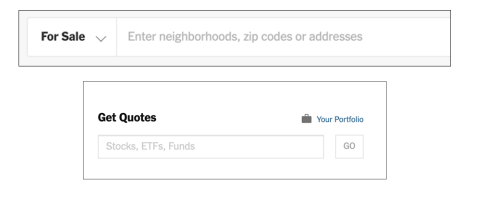
\includegraphics[scale=0.6]{images/lec08-pic31.png}
		\caption{Two search felds in the New York Times website hint at the variety of possible formats they will accept}
	\end{figure}	
\end{frame}

\begin{frame}[t]{Forgiving Format}
	\begin{figure}[h]
		\centering
		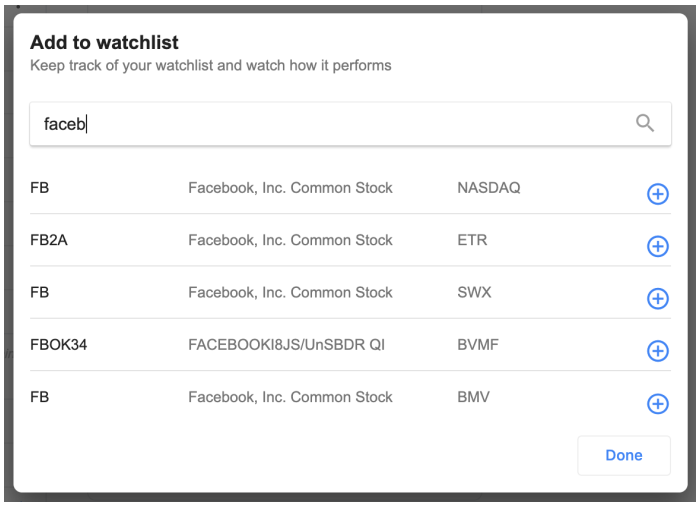
\includegraphics[scale=0.6]{images/lec08-pic32.png}
		\caption{Adding a stock to a personal watchlist in Google Finance}
	\end{figure}
\end{frame}

\begin{frame}[t]{Forgiving Format}
	\begin{figure}[h]
		\centering
		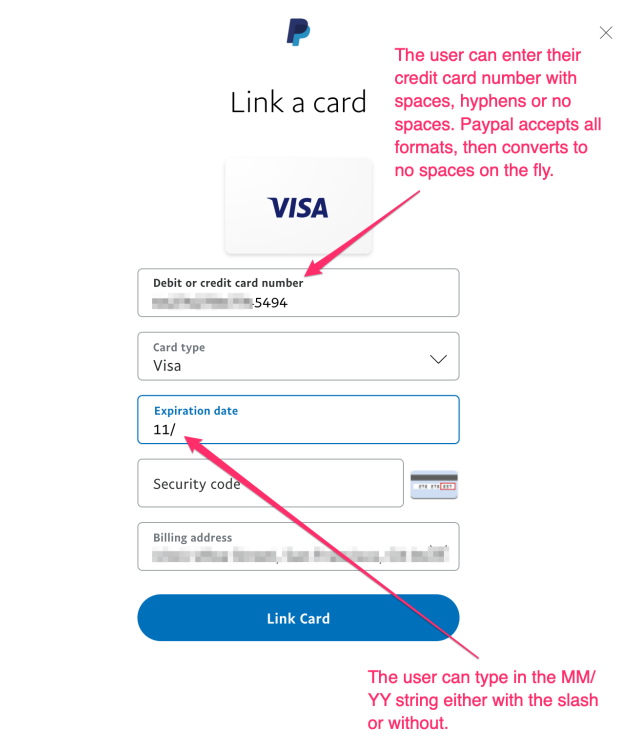
\includegraphics[scale=0.6]{images/lec08-pic33.png}
		\caption{PayPal}
	\end{figure}
\end{frame}

\begin{frame}[t]{Forgiving Format}
	\begin{figure}[h]
		\centering
		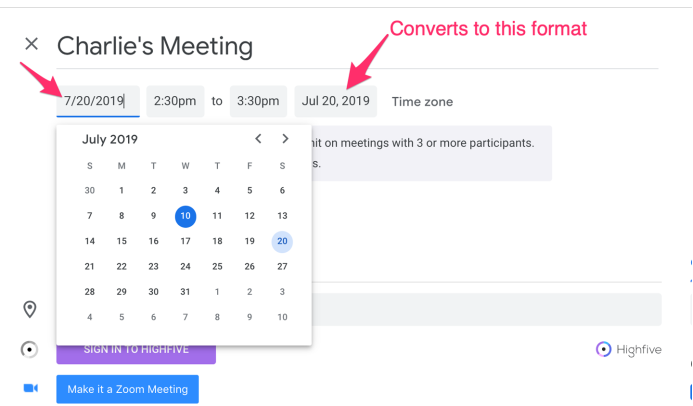
\includegraphics[scale=0.6]{images/lec08-pic34.png}
		\caption{Google Calendar}
	\end{figure}
\end{frame}

\begin{frame}[t]{Structured Format}
	\begin{figure}[h]
		\centering
		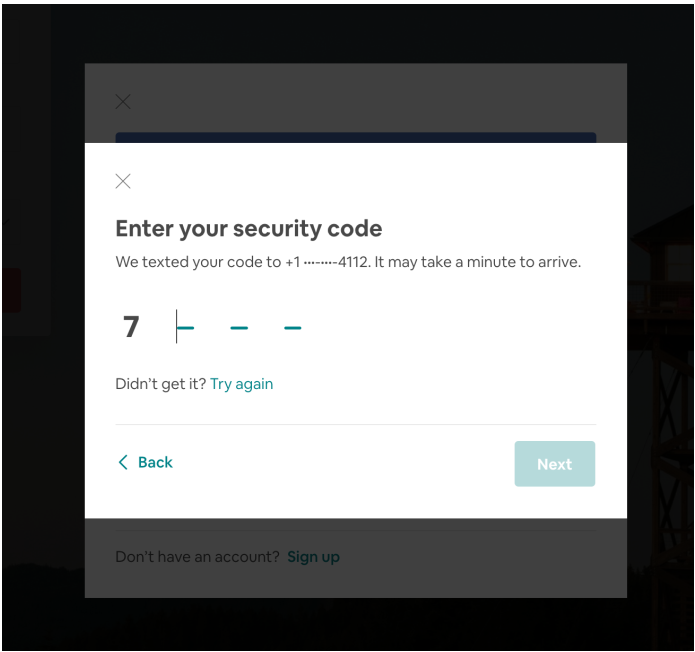
\includegraphics[scale=0.6]{images/lec08-pic35.png}
		\caption{Airbnb security code entry form}
	\end{figure}
\end{frame}

\begin{frame}[t]{Structured Format}
	\begin{figure}[h]
		\centering
		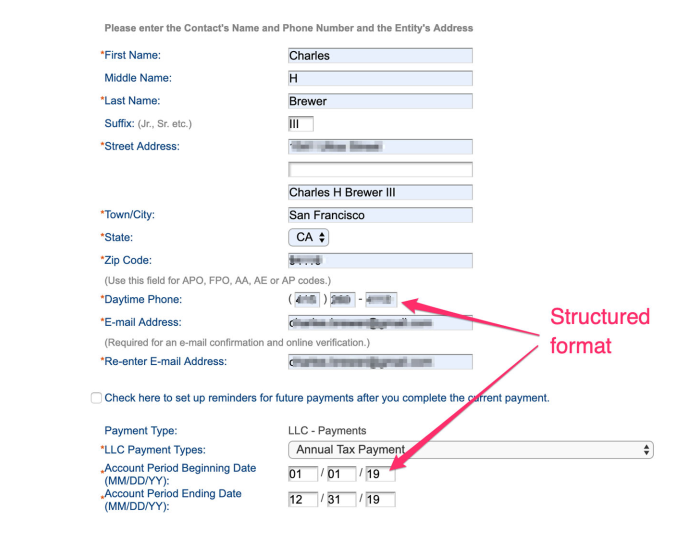
\includegraphics[scale=0.6]{images/lec08-pic36.png}
		\caption{Ocialpayments.com}
	\end{figure}
\end{frame}

\begin{frame}[t]{Structured Format}
	\begin{figure}[h]
		\centering
		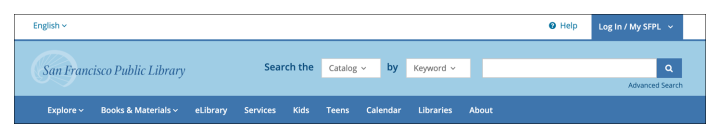
\includegraphics[scale=0.6]{images/lec08-pic37.png}
		\caption{San Francisco Public Library}
	\end{figure}
\end{frame}

\begin{frame}[t]{Structured Format}
	\begin{figure}[h]
		\centering
		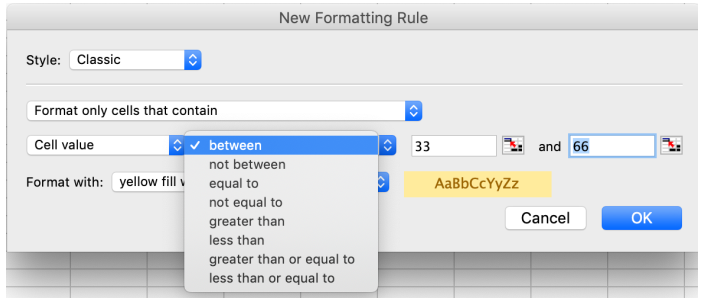
\includegraphics[scale=0.6]{images/lec08-pic38.png}
		\caption{Classic conditional fomatting in Microsof Excel}
	\end{figure}
\end{frame}

\begin{frame}[t]{Structured Format}
	\begin{figure}[h]
		\centering
		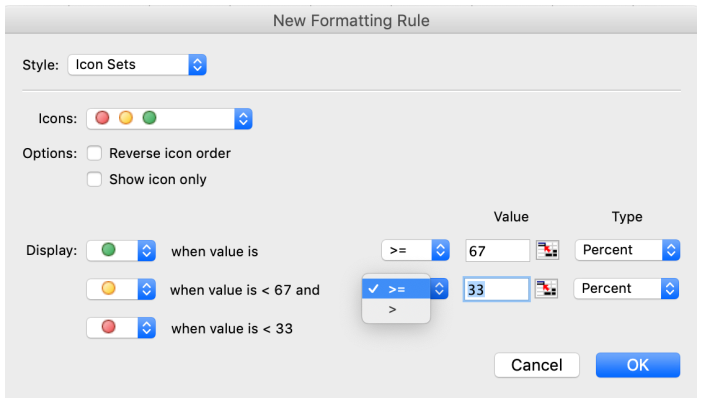
\includegraphics[scale=0.6]{images/lec08-pic39.png}
		\caption{Icon Set conditional formatting in Microsof Excel}
	\end{figure}
\end{frame}

\begin{frame}[t]{Structured Format}
	\begin{figure}[h]
		\centering
		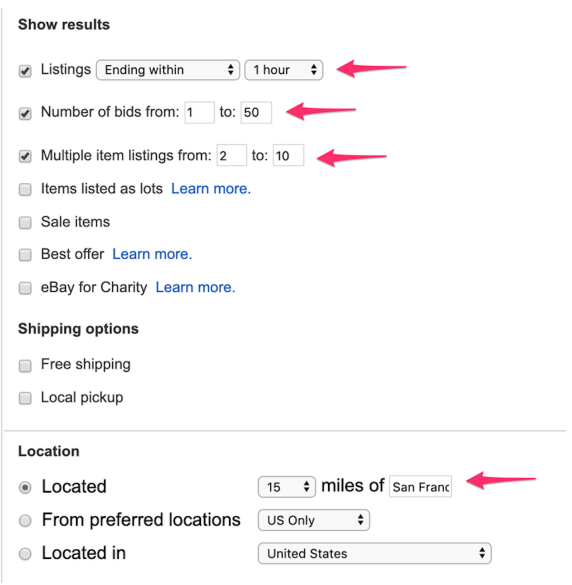
\includegraphics[scale=0.6]{images/lec08-pic40.png}
		\caption{eBay search flter form}
	\end{figure}
\end{frame}

\begin{frame}[t]{Input Hints}
	\begin{figure}[h]
		\centering
		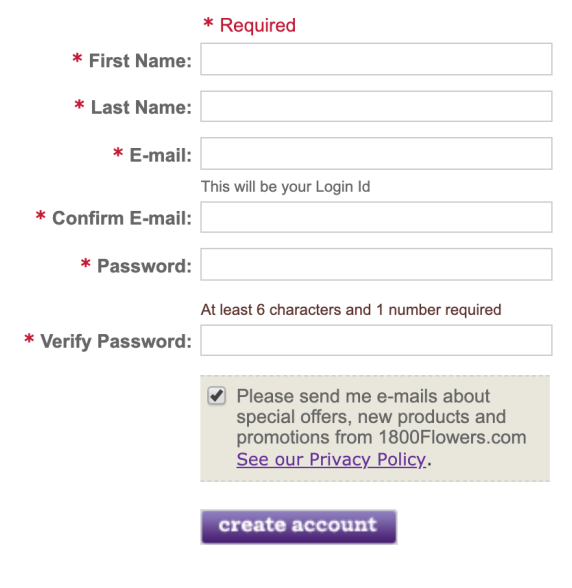
\includegraphics[scale=0.6]{images/lec08-pic41.png}
		\caption{The 1-800-Flowers registration screen}
	\end{figure}
\end{frame}

\begin{frame}[t]{Input Hints}
	\begin{figure}[h]
		\centering
		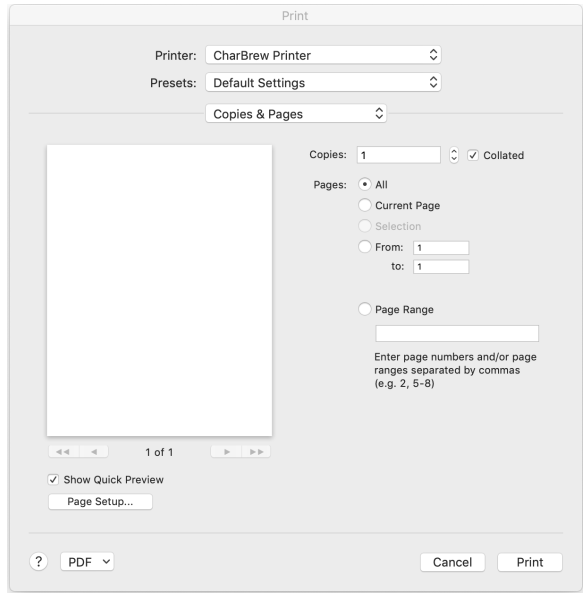
\includegraphics[scale=0.6]{images/lec08-pic42.png}
		\caption{Microsof Word print dialog box}
	\end{figure}
\end{frame}

\begin{frame}[t]{Input Hints}
	\begin{figure}[h]
		\centering
		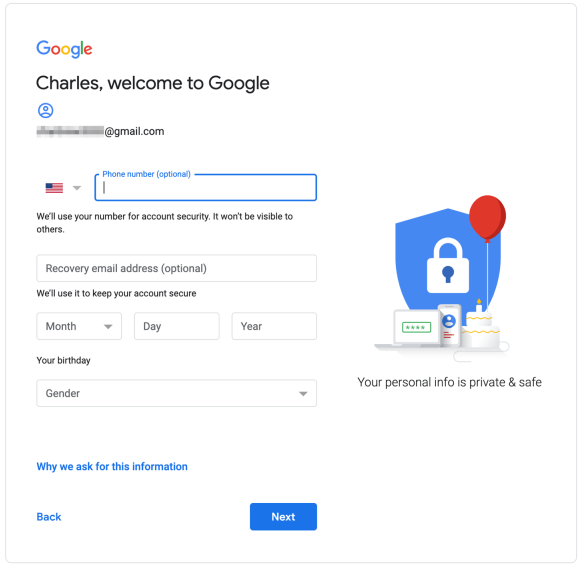
\includegraphics[scale=0.6]{images/lec08-pic43.png}
		\caption{Gmail registration page}
	\end{figure}
\end{frame}

\begin{frame}[t]{Input Hints}
	\begin{figure}[h]
		\centering
		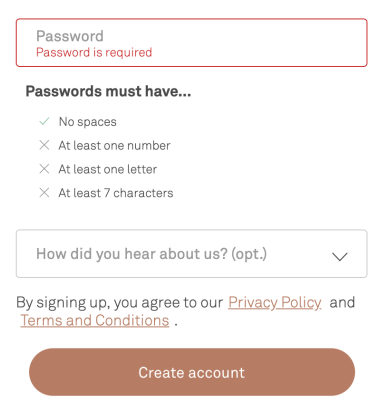
\includegraphics[scale=0.6]{images/lec08-pic44.png}
		\caption{Gmail registration page}
	\end{figure}
\end{frame}

\begin{frame}[t]{Input Hints}
	\begin{figure}[h]
		\centering
		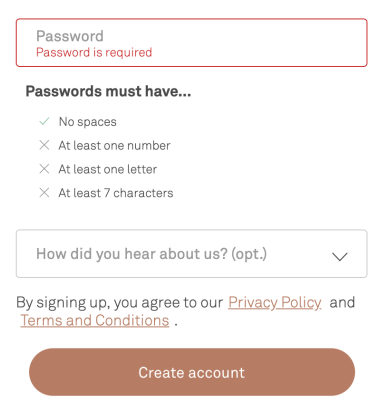
\includegraphics[scale=0.6]{images/lec08-pic45.png}
		\caption{Trunk Club}
	\end{figure}
\end{frame}

\begin{frame}[t]{Input Prompt}
	\begin{figure}[h]
		\centering
		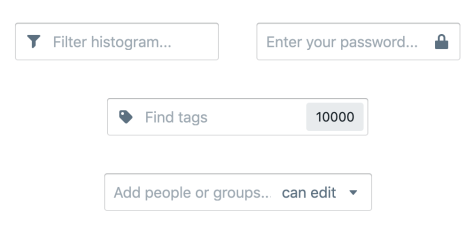
\includegraphics[scale=0.6]{images/lec08-pic46.png}
		\caption{Blueprintjs UI Toolkit; four example inputs with prompts}
	\end{figure}
\end{frame}

\begin{frame}[t]{Input Prompt}
	\begin{figure}[h]
		\centering
		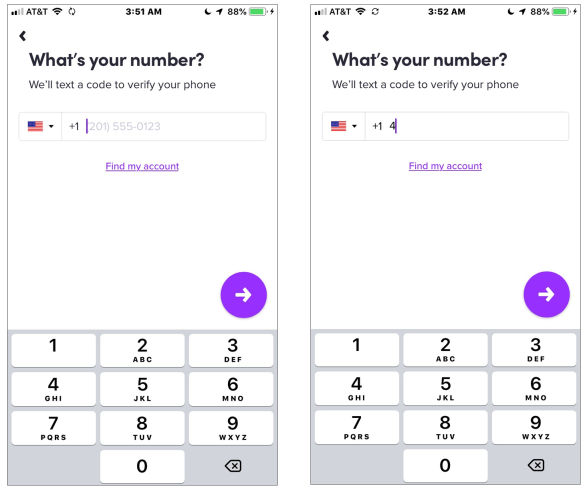
\includegraphics[scale=0.6]{images/lec08-pic47.png}
		\caption{Lyft mobile app input prompt}
	\end{figure}
\end{frame}

\begin{frame}[t]{Password Strength Meter}
	\begin{figure}[h]
		\centering
		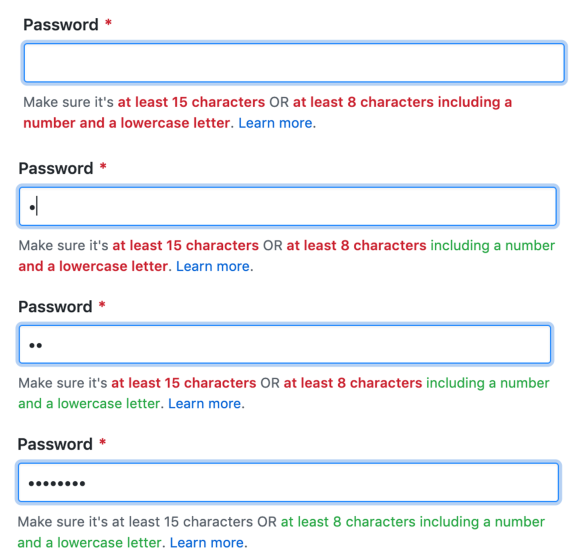
\includegraphics[scale=0.6]{images/lec08-pic48.png}
		\caption{GitHub password strength meter states}
	\end{figure}
\end{frame}

\begin{frame}[t]{Password Strength Meter}
	\begin{figure}[h]
		\centering
		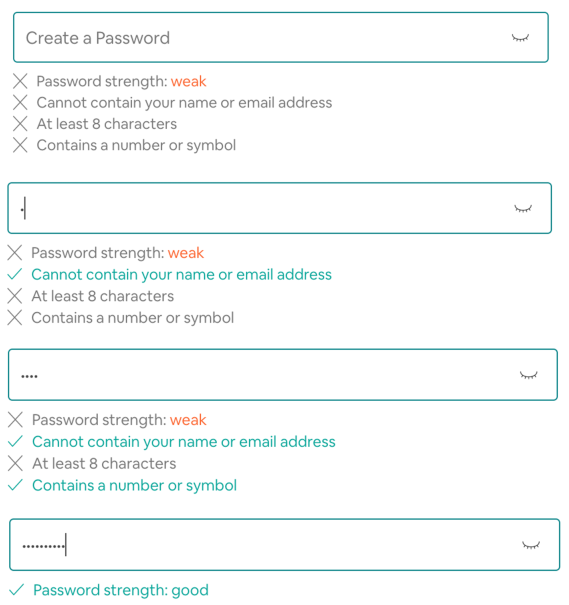
\includegraphics[scale=0.6]{images/lec08-pic49.png}
		\caption{Airbnb password strength meter states}
	\end{figure}
\end{frame}

\begin{frame}[t]{Autocompletion}
	\begin{figure}[h]
		\centering
		\includegraphics[scale=0.6]{images/lec08-pic50.png}
		\caption{Amazon autocomplete}
	\end{figure}
\end{frame}

\begin{frame}[t]{Autocompletion}
	\begin{figure}[h]
		\centering
		\includegraphics[scale=0.6]{images/lec08-pic51.png}
		\caption{Amazon autocomplete}
	\end{figure}
\end{frame}

\begin{frame}[t]{Autocompletion}
	\begin{figure}[h]
		\centering
		\includegraphics[scale=0.6]{images/lec08-pic52.png}
		\caption{Amazon autocomplete}
	\end{figure}
\end{frame}

\begin{frame}[t]{Autocompletion}
	\begin{figure}[h]
		\centering
		\includegraphics[scale=0.6]{images/lec08-pic53.png}
		\caption{Amazon autocomplete}
	\end{figure}
\end{frame}

\begin{frame}[t]{Autocompletion}
	\begin{figure}[h]
		\centering
		\includegraphics[scale=0.6]{images/lec08-pic54.png}
		\caption{Amazon autocomplete}
	\end{figure}
\end{frame}

\begin{frame}[t]{Autocompletion}
	\begin{figure}[h]
		\centering
		\includegraphics[scale=0.6]{images/lec08-pic55.png}
		\caption{Amazon autocomplete}
	\end{figure}
\end{frame}

\begin{frame}[t]{Drop-down Chooser}
	\begin{figure}[h]
		\centering
		\includegraphics[scale=0.6]{images/lec08-pic56.png}
		\caption{Microsof Word drop-down choosers}
	\end{figure}
\end{frame}

\begin{frame}[t]{Drop-down Chooser}
	\begin{figure}[h]
		\centering
		\includegraphics[scale=0.6]{images/lec08-pic57.png}
		\caption{1}
	\end{figure}
\end{frame}

\begin{frame}[t]{List Builder}
	\begin{figure}[h]
		\centering
		\includegraphics[scale=0.6]{images/lec08-pic58.png}
		\caption{1}
	\end{figure}
\end{frame}

\begin{frame}[t]{List Builder}
	\begin{figure}[h]
		\centering
		\includegraphics[scale=0.6]{images/lec08-pic59.png}
		\caption{1}
	\end{figure}
\end{frame}

\begin{frame}[t]{Good Defaults and Smart Prells}
	\begin{figure}[h]
		\centering
		\includegraphics[scale=0.6]{images/lec08-pic60.png}
		\caption{1}
	\end{figure}
\end{frame}

\begin{frame}[t]{Good Defaults and Smart Prells}
	\begin{figure}[h]
		\centering
		\includegraphics[scale=0.6]{images/lec08-pic61.png}
		\caption{1}
	\end{figure}
\end{frame}

\begin{frame}[t]{Good Defaults and Smart Prells}
	\begin{figure}[h]
		\centering
		\includegraphics[scale=0.6]{images/lec08-pic62.png}
		\caption{1}
	\end{figure}
\end{frame}

\begin{frame}[t]{Error Messages}
	\begin{figure}[h]
		\centering
		\includegraphics[scale=0.6]{images/lec08-pic63.png}
		\caption{1}
	\end{figure}
\end{frame}

\begin{frame}[t]{Error Messages}
	\begin{figure}[h]
		\centering
		\includegraphics[scale=0.6]{images/lec08-pic64.png}
		\caption{1}
	\end{figure}
\end{frame}

\begin{frame}[t]{Error Messages}
	\begin{figure}[h]
		\centering
		\includegraphics[scale=0.6]{images/lec08-pic65.png}
		\caption{1}
	\end{figure}
\end{frame}

\begin{frame}[t]{Error Messages}
	\begin{figure}[h]
		\centering
		\includegraphics[scale=0.6]{images/lec08-pic66.png}
		\caption{1}
	\end{figure}
\end{frame}

\end{document}
